\section{Results}
\label{sec:results}

We look for our usage patterns in our benchmark collection of 11 libraries (Table~\ref{tab:libs}).

\subsection{API bypasses}
We first investigate the use of API bypasses in our clients. This is useful to library developers if they want to identify which parts of their libraries that are supposed to be internal are actually used by clients. This can help them with API design in future versions. 

In Section~\ref{sec:classification}, we enumerate three broad categories
of bypasses: access modifiers, modularity conventions, and service loaders. We discuss each of them in turn.

%\input{tables/results/set-accessible-client-to-lib}
%\input{tables/results/set-accessible-lib-to-client}

\paragraph{Access modifiers and reflection}
Table~\ref{tab:set-accessible-client-to-lib}
shows selected uses of the reflection API \texttt{setAccessible()} to enable reflective access from clients to libraries,
and Table~\ref{tab:set-accessible-lib-to-client} shows selected uses of \texttt{setAccessible()} to enable reflective callbacks from libraries back to clients.
We can see that accesses to fields, constructors, and methods are all reasonably common, though some codebases only reflectively 
access fields, while others only access methods.

In our data, 1.9\% of the \texttt{setAccessible()} calls are 
used to ensure accessibility of a class member
in the same \texttt{rocketmq} project version 4.9.1 but in a different module (Maven module). 
For instance, \texttt{rocketmq-acl} makes private field \texttt{SendMessageRequestHeaderV2::a} from 
\texttt{rocketmq-common} accessible before accessing it. Such inter-module accesses are more controlled than client/library accesses since they are within the same project,
but are still a form of technical debt.

We investigated all \texttt{setAccessible()} calls on fields that belong to in \emph{rocketmq}. (\emph{rocketmq} is a client that calls \emph{fastjson}). These calls are made from the library to the client, i.e., accesses are from library \emph{fastjson} to client \emph{rocketmq} using callbacks. We see hundreds of \texttt{setAccessible()} calls being executed when the client tests are run. The \emph{rocketmq} source code shows 6 classes with calls to \texttt{setAccessible()}: a serialization/deserialization pair for the \texttt{CommandCustomHeader} class, 2 methods which appear to print out the state of an object for debugging or logging purposes, and 2 methods which store a reference to a specified field or which call a specified method, provided in those methods' parameters. We would not characterize the first 4 API bypasses as misuses, and it is not obvious that the last 2 are misuses either. Another interesting use of \texttt{setAccessible()} on a field is by \emph{benchmark-thrift} to access the field \texttt{maxLength\_}  which is a class member of the class \texttt{TFramedTransport} belonging to Apache \emph{thrift}. This is a private field and the default maximum length is overridden by the client.

We found that 23\% of the calls to \texttt{setAccessible()} were on methods. Of those, only 2 distinct methods that were reflectively invoked were previously not accessible. We manually inspected all of the reflective callers of these 2 methods. Protected method \texttt{Node.setParentNode()} in \emph{jsoup} is called from code in \texttt{org.seimicrawler.xpath} in \emph{JsoupXpath}. This appears to be test code committed to the main repository. The next method is the default-visibility method \texttt{getInstance()}. This method is used to obtain a singleton instance of {\tt ReflectionNavigator} from within the same project. The motivation for developers calling \texttt{setAccessible} within the same project is unclear to us, rather than modifying the code themselves. This work can help developers identify such instances and possibly refactor their code.

We do find that some methods are already accessible before being invoked, and some methods are made accessible but never actually invoked.

An API bypass requires a \texttt{setAccessible()} call followed by an
actual reflective access.  As expected, we see a good overlap between the
\texttt{setAccessible()} calls to methods and reflective invocations.
We find that our benchmarks contain reflective invocations of 20 constructors following a call to \texttt{setAccessible}, which were not already public. Of the 20 callsites, some are generated by the
groovy dynamic language; some are for serialization and some instantiate objects where the constructor had default visibility. All of these reflective constructor invocations are callbacks from the library to the client: the library is providing a factory method to create instances of a client type that it has been supplied with. This appears to be an acceptable API use.
Tables~\ref{tab:refl-fields} and \ref{tab:refl-callbacks} show how many reflective usages are actually made.

Table~\ref{tab:refl-fields} shows some of our data on reflective field accesses. We observe that many of these reflective field accesses are for serialization. We also observe that in the case of fields, there are only a few calls that access fields that were previously not accessible.
%\input{tables/results/reflective-fields}

Table~\ref{tab:refl-callbacks} shows the reflective callback API usage pattern. We see that most accesses in this pattern are made on public methods. We examined the list of methods that are accessed using this usage pattern and this pattern is popular for logging, serialization and deserialization. We also observe a lot of getters and setters accessed this way.



%\input{tables/results/reflective-invocations-client-to-lib}


%% facts about methods:
%% # 827
%% protected 1 org.seimicrawler.xpath.core.node.Text$1::head(Lorg/jsoup/nodes/Node;I)V to org.jsoup.nodes.Node::setParentNode(Lorg/jsoup/nodes/Node;)V, looks like test code
%% default 3 com.sun.xml.bind:jaxb-core:2.2.11 to com.sun.xml.bind.v2.model.nav.ReflectionNavigator::getInstance()Lcom/sun/xml/bind/v2/model/nav/ReflectionNavigator;

%% many of the other calls are during serialization


%% Similarly, \texttt{setAccessible()} on methods in \emph{fastjson} at the behest of \emph{rocketmq} is on constructors, factory methods, and build methods, in the context of Java Beans. As with the fields, these calls essentially enable serialization and deserialization, and are made from class JavaBeanDeserializer.

%% \todo[inline]{Our hypothesis: setAccessible() on methods is used almost exclusively in tests and in serialization. We can verify this by filtering the setAccessible() method calls and excluding everything with ``Test'' and ``Bean'' in it.}
%\input{tables/results/reflective-callbacks}

\paragraph{Containers, modules, and modularity conventions}
For OSGi, none of our libraries are used by our clients in the context of OSGi containers, so the clients are free to violate OSGi access control. Our results show that, even though they can, they almost universally do not. The sole exception is a pair of calls from client \texttt{xsoup} to internal class \texttt{StringUtil} of library \texttt{jsoup}; the calling class in \texttt{xsoup} was copied from \texttt{jsoup} and still uses its internal helper functions. These calls violate both modularity conventions and OSGi export declarations. When we found these calls, we submitted a pull request\footnote{https://github.com/code4craft/xsoup/pull/53} duplicating the \texttt{jsoup} methods into \texttt{xsoup}, and it was quickly merged, showing that the \texttt{xsoup} developer was not in favour of violating modularity conventions.
% https://github.com/code4craft/xsoup/pull/53

Similarly, although we have Java 8 clients which can violate the unenforced module export rules of Java 9 libraries (they run in environments that don't enforce the rules), none of the clients do so. We believe that the most likely explanation is that such modularity violations are uncommon; however, it is also possible that Java 9 module definitions are too permissive and do not prevent calls that should be prevented.

Table~\ref{tab:internal} shows uses of packages labelled ``internal'' from outside
a given module. In some cases (for example, netty-buffer and netty-common),
the uses are across different modules in the same project. We looked
at one case, \emph{rocketmq-remoting} and \emph{netty}. In this case,
\emph{rocketmq-remoting} uses internal logging infrastructure from
\emph{netty} in its NettyLogger module; such a module might be
expected to be more closely coupled to its callee than other parts of
the code. On the other hand, the usage of \emph{groovy} internals in
\emph{rest-assured} would appear to be due to the choice of Groovy as
an implementation language, and thus compiler-generated references to
internals in the \emph{rest-assured} code.

%\input{tables/results/internal}


\paragraph{Service bypasses}
We find that all clients of libraries that use service loaders bypass the defined services. This is done most commonly through instantiation, but also through casts, subtyping and reflection.

For instance, component \emph{com.h2database:h2} advertises a service (\texttt{org.h2.Driver} implementing \texttt{java.sql.Driver}), making it a JDBC4-compliant driver. Its clients can obtain connections through the JDBC driver manager, which selects and instantiates instances based on driver URLs. However, client \texttt{glowroot.agent} (specifically class \texttt{org.glowroot.\-agent.embedded.util.DataSource}) directly instantiates \texttt{org.h2.jdbc.JdbcConnection} and therefore becomes dependent on using the particular database \emph{h2}. This leads to further direct calls to \texttt{org.h2.jdbc} APIs being observed. This is a clear bypass of a defined API. 

Now consider \emph{fastjson}. This component declares that it provides several services, including three services defined by interfaces in the \texttt{javax.ws.rs.ext} package, part of the JEE support for RESTful services. 
The respective services are implemented in classes in the package \texttt{com.alibaba.fastjson.support.jaxrs}.   
However, looking at clients, we also see calls to APIs provided in \emph{fastjson} APIs outside packages implementing the interfaces declared as services. For instance, \texttt{com.alibaba.fastjson.JSON::toJSONString} is called from \texttt{org.springframework:spring-web}.
%:4.3.7.RELEASE.    
This is a legitimate use of a JSON parser via a non-standard API, and in this sense, it is a false positive as we detect it as a API misuse. So \emph{fastjson} could be easily split into two components, one providing an ``open API'' for the JSON parser functionality, and one implementing and providing the RESTful services. The services would then depend on the open API. This would significantly reduce the overall API surface of fastjson, splitting it into two components, each with well defined functionalities and internal coherence.

We have mainly focussed on ``why not'', i.e. what mechanisms clients use to bypass API restrictions: reflection, violating conventions, and service loader bypasses, and reported results with respect to ``what thing''. When relevant, we discussed ``how'' the bypass occurred, especially for reflection, and we reported the directionality of the bypasses.

\begin{mdframed}[
  leftmargin=\parindent,
  rightmargin=\parindent,
  skipabove=\topsep,
  skipbelow=\topsep
  ]
{\bf Finding 1:} Programs are generally well-behaved: reflection is mostly used for serialization not API bypasses; OSGi and Java 9 module definitions are always respected; internal packages are only called sparingly; but service loaders are almost always bypassed.
\end{mdframed}

\subsection{Extent of API usage}
Continuing with our investigation of API surfaces, but moving from
misuses to uses, we present results on API use.
%, again using results obtained from our instrumentation.

Table~\ref{tab:usage-distribution} presents the usage distribution of
libraries' API elements (methods, fields, and classes subtyped) as
covered by client tests. The ``total in lib'' refers to the number of
public and protected members, including static ones. To calculate these totals,
we use the latest stable version of each library and consider it to be representative of 
the versions used by clients.  The ``distinct used'' column counts an
element once regardless of how many clients use that element, while
``total used'' counts an element once per client using it. We identify method calls by the
declared type of the receiver object, for example, calls to {\tt o1.f()} and {\tt o2.f()} are the same
if {\tt o1} and {\tt o2} have the same declared type.
Our uses 
include both vanilla and reflective uses of API elements.

%\input{tables/results/standard-api-usage}

We can observe that at most 22\% (and on average 9\%) of the methods in the API surface
are used by clients, with \emph{slf4j-api} having the highest use proportion.
% , and sometimes less than 1\%  of methods. 
Table~\ref{tab:usage-distribution} suggests that there is a small overlap between methods
used by clients.

We also looked at the \emph{json} library and found that its own tests reach 151
of the 258 API methods, compared to the 25 methods used by our selected
clients. One possible reason for the sparsity of API use is that, at least in \emph{json}, over half of the API methods are overloaded, i.e. share a name with
some other API method.

% reads or writes would be nice to know, but we can't get it in time.
Despite standard OO practices calling for fields to be encapsulated, more than half of the libraries have their fields accessed by clients. Only 1 of the \emph{joda-time} and 25 of the \emph{jackson-core} fields are static (so it's not just constants); the rest of the accesses are to instance fields.
However, the number of fields used is often in the single digits,
the \emph{jackson} libraries being an exception with about 11\% of declared fields used.
We inspected the use of \emph{jackson} fields and found that these usages mostly exist within the \emph{jackson} libraries themselves.
We count calls that happen across the \emph{jackson} libraries as crossing library/client boundaries.
An example of these usages is the {\tt WritableTypeId} class belonging to \emph{jackson-core}, which is used often, and usually by \emph{jackson-databind}.
{\tt WritableTypeId} is a Java class that acts like a C-style struct; it exposes fields and not methods. It is intended to be used for passing information, and the use of its fields is expected.

About half of the libraries have clients subclassing a
single-digit number of library types, again with the exception of
\emph{jackson} with dozens of subtypes in clients, which are also often other \emph{jackson} libraries.

We observe only one use of library annotations across all our benchmarks. \emph{crushpaper} uses \texttt{com.fasterxml.jackson.databind.annotation.JacksonStdImpl}, which is used for indicating implementation classes and is typically used by serializers and deserializers in \emph{jackson}.

Figure~\ref{fig:jaccard} presents a boxplot of
pairwise Jaccard similarities between the portion of
the APIs used by different clients for each library. Two clients $u_1$ and $u_2$ 
of library $L$ which use exactly the same parts of $L$'s API would result in a similarity of 1;
more generally, it is
\[ \frac{|\mbox{used.API}_L(u_1) \cap \mbox{used.API}_L(u_2)|}{|\mbox{used.API}_L(u_1) \cup \mbox{used.API}_L(u_2)|}. \]

Although Table~\ref{tab:usage-distribution} showed that some of the members overlap, we can
see from this Figure that the overall level of overlap is generally less than 10\%. We observe
a half-dozen client pairs (data points) where there is about 50\% overlap between client API uses, including for \emph{fastjson},
\emph{commons-io}, and \emph{json}. Although the mean overlap for \emph{slf4j-api} is near 0, there are also 4 pairs of clients which have more than 50\% overlap.

\begin{center}
\begin{figure}
\centering
%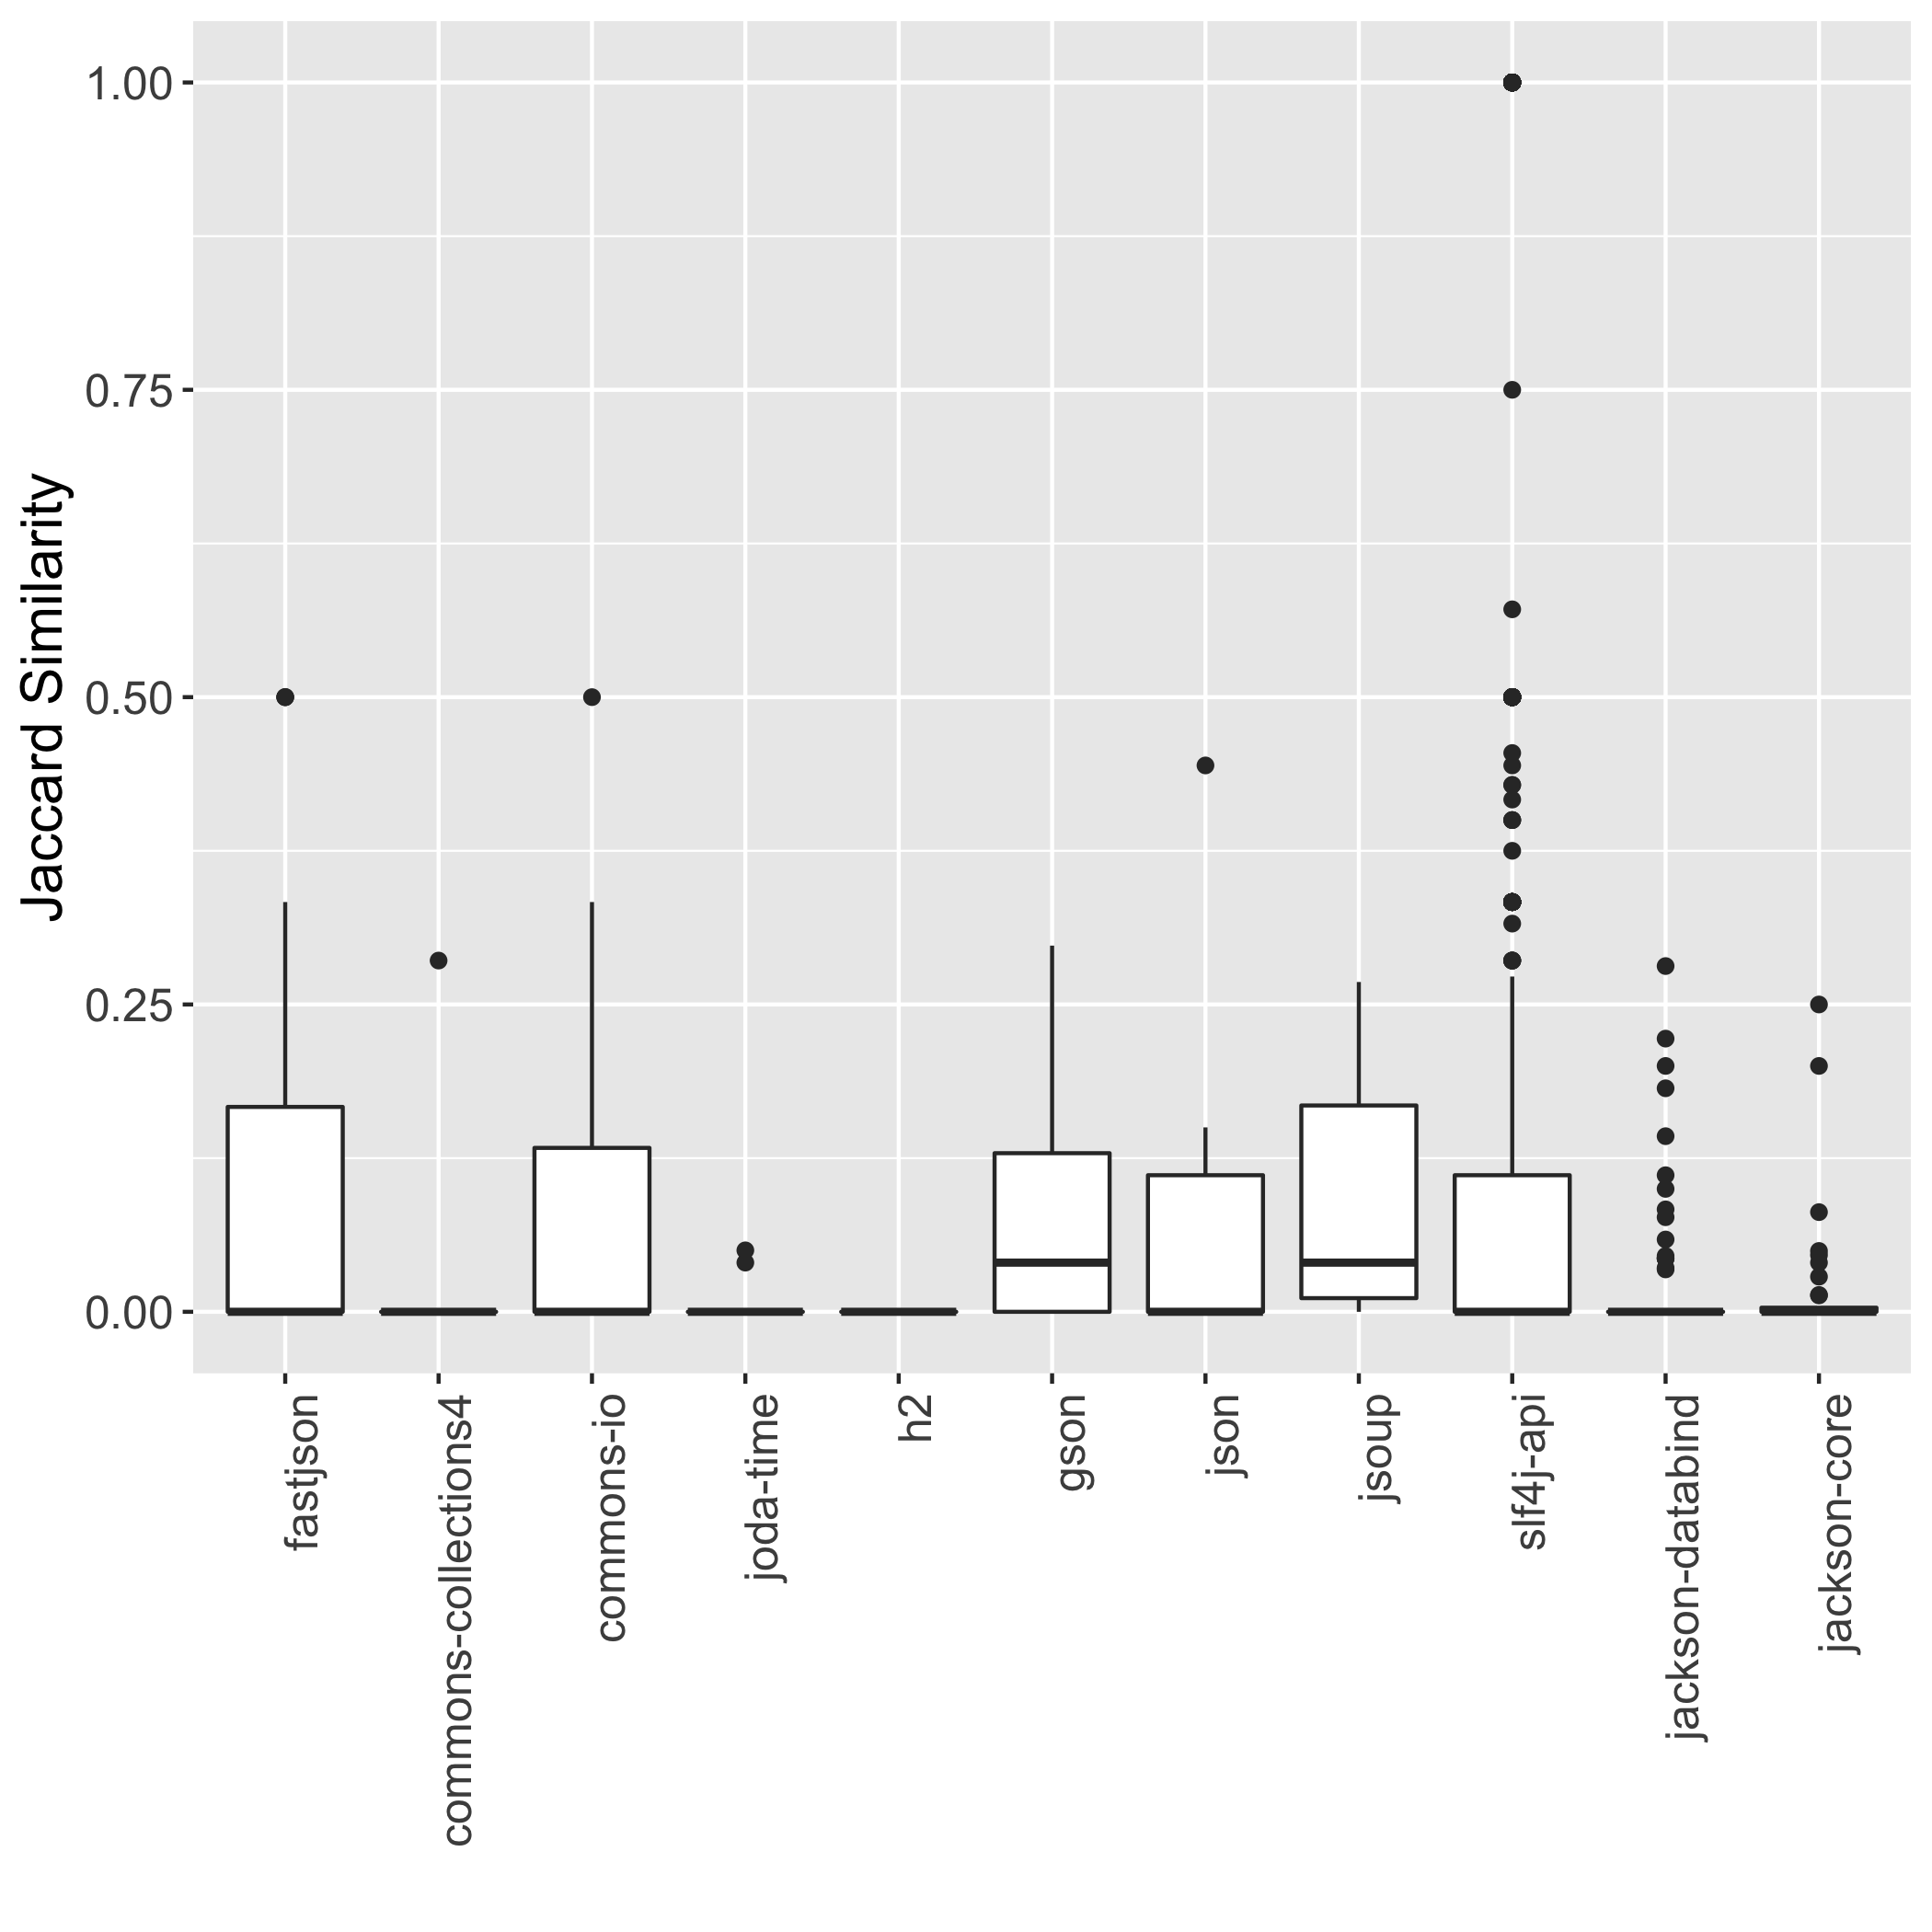
\includegraphics[width=8cm, height=7cm]{./images/jac-sim-box-plot-declared}
\caption{\label{fig:jaccard}Jaccard similarities between clients' API usages}
\end{figure}
\end{center}
%% Digging into \emph{fastjson}, we found that it is a ``mixed type'' library: some clients use APIs related
%% to \texttt{javax.ws.rs}, the JEE standard for restful services, while others use just a standalone parser API that does not implement an external specification. 

We were not surprised by the generally small amounts of overlap, because the libraries' exposed API surfaces tended
to have thousands of exposed elements and hundreds of used elements. This result makes a convincing argument for libraries being fissioned into modules, which we discuss further in Section~\ref{sec:fission}. 

Table~\ref{tab:same-method} presents another view of API overlap between clients. We constructed the largest set
of methods shared by more than 1 client of a library (``max-set'') and report the size of that set as well as the percentage
of clients which use all of that set of methods. So, for \emph{json}, we can see that there is one method called
by 3 out of 4 clients, and for \emph{jsoup}, ten methods are all called
by 3 out of 4 clients. We characterize the amount of overlap as generally low but not
nonexistent: a few methods are repeatedly used.

%\input{tables/results/perc-clients-same-methods}

%{\bf Research Question 2.} (a) Do clients often use only a subset of the published API? How big is this subset? (b) For each library, is that subset consistent across clients? (c) Do different libraries show different usage patterns by clients?

\begin{mdframed}[
  leftmargin=\parindent,
  rightmargin=\parindent,
  skipabove=\topsep,
  skipbelow=\topsep
  ]
{\bf Finding 2:} APIs are sparsely used by clients---mostly methods (9\% utilization), but a few fields (4\%) and supertypes (6\%). There is limited but nonzero overlap between the methods used by different clients.
\end{mdframed}
